% Project 2 - EECS 499
% Author: Shaun Howard (smh150@case.edu)
\documentclass[conference]{IEEEtran} \usepackage[T1]{fontenc} \usepackage[backend=biber, style=ieee]{biblatex}
\addbibresource{report.bib} \usepackage[final]{microtype}

% graphics
\ifCLASSINFOpdf \usepackage[pdftex]{graphicx} % declare the path(s) where your graphic files are
  \graphicspath{{images/}} % and their extensions so you won't have to specify these with
  % every instance of \includegraphics
  \DeclareGraphicsExtensions{.jpeg,.png} \else
\fi

\usepackage{amsmath}
\usepackage[linesnumbered,ruled]{algorithm2e}
\usepackage{comment}
\usepackage[noend]{algpseudocode}

\newcommand{\sfunction}[1]{\textsf{\textsc{#1}}}
\algrenewcommand\algorithmicforall{\textbf{foreach}}
\algrenewcommand\algorithmicindent{.8em}

\begin{document}

\title{Turtlebot OMPL Motion Planner Benchmark}

\author{
 \IEEEauthorblockN{Shaun Howard}
 \IEEEauthorblockA{Electrical Engineering and Computer Science Department\\
                   Case Western Reserve University\\ 
                   Cleveland, Ohio 44106\\
                   Email: smh150@case.edu}
}

% make the title area
\maketitle

% As a general rule, do not put math, special symbols or citations
% in the abstract
\begin{abstract}
Motion planning is an important part of modern robotics. Motion plans are intricate and sometimes time-consuming to develop in real scenarios.
The modern abstraction of motion planning has left most researchers to focus on new things. However, sometimes we take for granted the solutions
we are given to problems that we encounter everyday. Although the solution we interpret as right might approximately solve the problem, it may not 
be the best solution available. This paper focuses on analysing the pros and cons of all the modern geometric planners OMPL has to offer in order to
determine the best choice where obstacle avoidance and complex path planning are necessary. We also explore their statistical similarities and differences using the OMPL 
Benchmark libraries. 
The goal of this paper is to determine if the planners we currently use in the robotics industry will be the best and most efficient choices for the 
tasks of tomorrow.
\end{abstract}

\section{Introduction} \label{Introduction}

The search for accurate and quick planning algorithms has grown in recent years with major breakthroughs in memory architecture, processing unit speed and 
parallel processing. Robots inherently have higher degrees of freedom and more dimensions of parameters to tweak in their environments.Several planning methods exist that 
intricately check environment surroundings, configuration space and workspace constraints, and validate
that solutions can be executed by the robot due to differential or joint limits and constraints. Current planners may or may not be able to cope with dynamic environment 
updates that are not predictable by some sort of probabilistic approach. Spontaneity in determining solutions within a small window of time is a valuable trait of a 
modern motion planner. Obstacles may have complex behaviours that many robots may not understand quick enough to react. Today, with autonomous vehicles on the rise, 
quicker and more accurate planners are needed to support continuous and dynamic behaviour.

Sampling-based motion planning techniques were developed to facilitate the search for new solutions in less time. These planners were developed to randomly explore the
high-dimensional search space of modern robots in order to spontaneously find unique solutions to problems. The idea of these planners is to randomly generate a graph
of possible nodes to explore for the robot, represented typically within a bounded workspace, and connect them from either direction, if possible, to reach the goal 
without collisions from start to finish. Sometimes, solutions are picked that meet the constraints of the given task being executed for some probability of the time, 
while the remainder of the time, the planner approaches the goal. Some planners can solve many problem queries from one graph. A primary single-query sampling-based approach to motion planning is the Rapidly-
exploring Random Tree (RRT). A primary multi-query sampling-based technique, used especially for driving, is the probabilistic roadmap (PRM). Improvements have been
made to both planning algorithms to allow for quicker and more compact motion plans such as the RRT*, LazyRRT, LazyPRM, Fast Marching Tree Star (FMT*) and SPARS
and SPARS2, which utilize a rendition of the PRM to enable quick planning with near optimal shortest paths. 

A straightforward way to test these algorithms and others would be to implement an instance 
of the Open Motion Planning Library (OMPL), as described by Șucan, Moll, and Kavraki in \cite{ompl}. The OMPL has several implementations of motion planning algorithms 
including those mentioned above. The OMPL Benchmark library, as presented in \cite{ompl_benchmark}, will be useful for benchmarking those algorithms and acquiring the
data necessary for benchmark comparison. The benchmark library will run each algorithm on each of the problem descriptions from start to goal locations. 
Experiments can thus be chained together to tremendously speed up benchmarking. 

The turtlebot simulator is an appropriate simulator model for OMPL benchmarking purposes. The turtlebot simulator environment and costmap are display in figure 1. 
Autonomous driving is a large focus in motion planning today and the turtlebot leans closer to the driving aspect of motion planning than does a humanoid-type simulation. 
Given the simplicity of physical turtlebot set-up, it will be highly generalizable to test on a robot that is common and easy to set-up for modern consumers. It will also 
be appropriate to constraint motion plans based on differential constraints of the turtlebot, as most vehicles similarly have. Overall, the AMCL planner with a generated 
map of a test turtlebot environment will be used for robot localization benchmarking purposes. The map will be represented to the robot by means of a 2-dimensional 
costmap, generated primarily by the dynamic window approach (DWA) planner provided by ROS. The DWA implemented by ROS is based on the methodology proposed by D. Fox, W. 
Burgard, and S. Thrun. in \cite{dwa}. The benchmarking planner will inherit properties from the BaseGlobalPlanner provided by ROS in order to act as a true motion 
planning plug-in for compatibility with components of the ROS motion planning framework like the Rviz robot interaction and visualization application.

The next sections describe the algorithms, outline their pros and cons, employ them in benchmark test scenarios and compare their experimentation results using 
statistical analysis.

\section{Planning Algorithms} \label{Planning Algorithms}

\subsection{Rapidly-Exploring Random Tree} \label{RRT}
The rapidly-exploring random tree algorithm was pioneered by S. LaValle and J. Kuffner around 2000. The RRT was designed to rapidly and randomly explore high-dimensional
state space in a completely configurable but always sampling-based method. They proved that it is probabilistically complete when they implemented it in their 2001 paper 
\cite{random_kinodynamics}, where they experiment with an under-actuated spacecraft that performs complex maneuvers amongst other robots and compare the performance 
results. The pseudocode for the algorithm is displayed in figure 2.

\begin{figure}
\label{figure2} 
\centering 
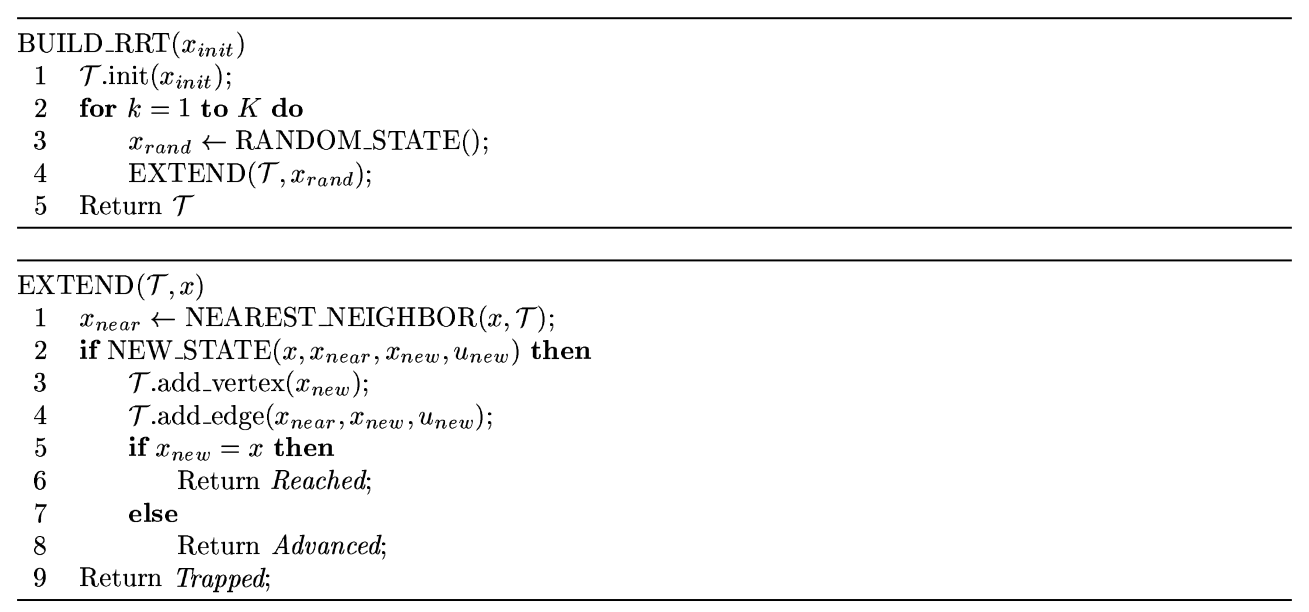
\includegraphics[width=0.49\textwidth]{rrt}
\caption{RRT pseudocode}
\end{figure}

The upsides to the RRT planner are the following:
-probabilistically complete
-performance
-no preprocessing
-simplification of higher dimensionality
-good with differential constraints
-good with nonlinear systems

The downsides of the RRT planner are the following:
-no memory for multiple queries
-optimality is not guaranteed

\subsection{RRT*} \label{RRT*}
The heuristically-driven RRT, RRT*, is a rendition of the RRT that uses a distance or obstacle-based cost heuristic to reach the goal. The RRT* is approximately 
asymptotically optimal, like the well-known A* algorithm. This version of the RRT planning algorithm was introduced in \cite{sampling_star}. Since the RRT* is almost
optimal, this means that the cost of the returned solution path converges almost definitely to the optimal solution for that planning problem. The pseudocode for the
RRT* algorithm is in figure 3.

\begin{figure}
\label{figure3} 
\centering 
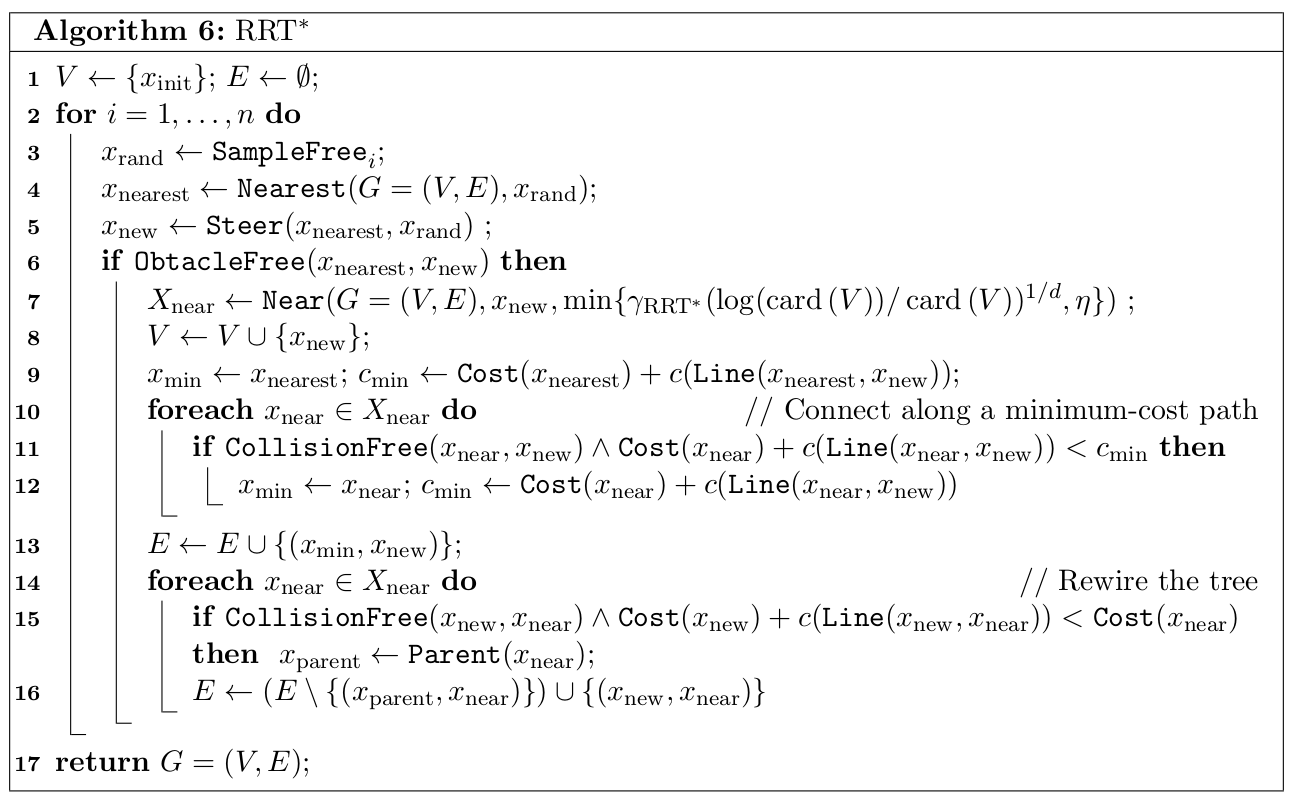
\includegraphics[width=0.49\textwidth]{rrt_star}
\caption{RRT* pseudocode}
\end{figure}

The pros of the RRT* algorithm follow:
-probabilistically complete
-asymptotically optimal
-monotone convergence

The cons of the RRT* algorithm follow:
-cons of RRT, such as no memory for solutions

\subsection{LazyRRT} \label{LazyRRT}
The lazy RRT is a rendition of the RRT that explores only part of the random tree that is necessary to solve the current query. It was first introduced by R. Bohlin and 
L. Kavraki in \cite{lazy_rrt}. The lazy RRT is an RRT optimized for single-query, high-dimensional, uncluttered, global configuration spaces. The lazy RRT aims to 
minimize the number of collision checks performed during the RRT planning process. This addition to the RRT makes for a more efficient implementation of the RRT that has 
a better runtime in the general case. The pseudocode for the LazyRRT algorithm is displayed in figure 4.

\begin{figure}
\label{figure4} 
\centering 
\includegraphics[width=0.49\textwidth]{lazy_rrt}
\caption{LazyRRT pseudocode}
\end{figure}

The good features of the LazyRRT are:
-speedup from reduced collision checking
-same as RRT

The bad features of the LazyRRT are:
-cons of RRT minus collision-checking inefficiencies
-worst case runtime matches RRT worst case runtime due to frequent collision checks

\subsection{Probabilistic Roadmap} \label{PRM}
The probabilistic roadmap was first released the to the public in 1996 with \cite{prm}. The goal was to build a map of possible nodes to visit amongst the obstacles in 
the environment. The algorithm is based on a static map of the robot's environment. The planner has two phases: a learning and a query phase. The nodes represent 
collision-free robot configurations, while the edges represent clear paths to travel between those nodes. The PRM is known to excel with the help of a local planner like 
the ROS DWA planner that will be used in this benchmark. The algorithm pseudocode is presented in figure 5.

\begin{figure}
\label{figure5} 
\centering 
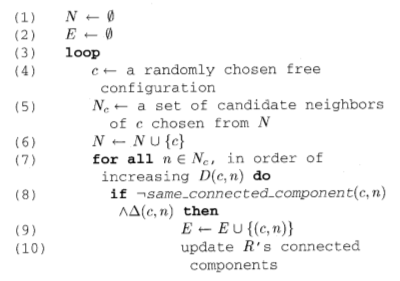
\includegraphics[width=0.49\textwidth]{prm}
\caption{PRM pseudocode}
\end{figure}

The pros of the PRM:
-probabilistically complete
-monotone convergence

The cons of the PRM:
-issues handling differential constraints
-not guaranteed to be asymptotically optimal
-slower query time that RRT
-inability to deal with environment changes without reconstruction

\subsection{LazyPRM} \label{LazyPRM}
The lazy PRM is an enhanced version of the PRM that lazily checks for collisions. The lazy PRM was described as an enhancement to the PRM in \cite{lazy_prm}. Initially, 
the planner assumes that all randomly-generated configurations are collision-free. Once nodes or edges with collisions are found, they are removed from the roadmap and
new nodes and/or edges are generated and inserted. This process is repeated until a collision-free solution is found. The theme of the planner is to minimize the number
of collision checks needed to reach a goal. The pseudcode of the LazyPRM is shown in figure 6.

\begin{figure}
\label{figure6} 
\centering 
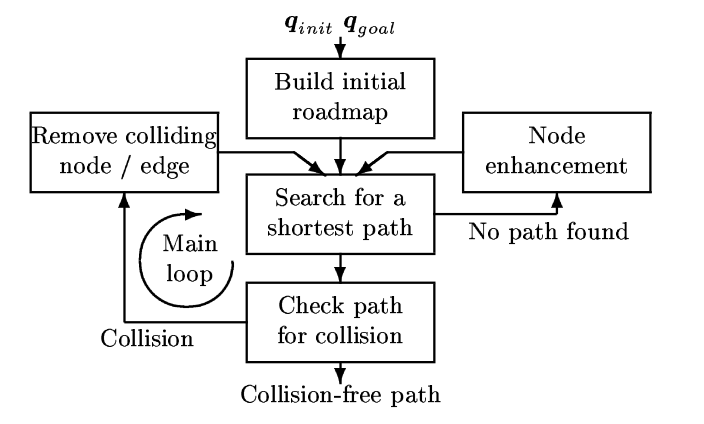
\includegraphics[width=0.49\textwidth]{lazy_prm}
\caption{LazyPRM pseudocode}
\end{figure}

The pros of the LazyPRM:
-pros of PRM
-speedup from infrequent collision checking

The cons of the LazyPRM:
-cons of PRM minus collision checking inefficiencies
-worst case runtime matches PRM worst case runtime due to frequent collision checks

\subsection{SPArse Roadmap Spanner Algorithm} \label{SPARS}
The SPARS planner is a divergence from the typical sampling-based PRM and heuristically-driven PRM star algorithms. The work in \cite{spars} develops a method of planning 
that shows finite-size data structures can have close to optimal properties without spanning over as much space as previously integrated PRM* graph spanners. Query
resolution for the SPARS planner is faster than for mainstream PRM*-based planners. Although most PRM algorithms require the map to grow infinitely large to converge to 
the desired state of optimality, the SPARS algorithm satisfies near-optimality, workspace bounds and completeness criteria to generate solutions much faster than typical
PRM planners, while benefiting from the same upsides of the PRM approaches. After smoothing, paths are found to be much shorter than paths developed by other algorithms.

The SPARS planner provides probabilistic completeness and near asymptotic optimality by building two graphs in parallel. The first graph is a dense asymptotically-optimal
PRM*-based roadmap and the second graphs is the spanner of the first graph. The SPARS pseudocode can be found in figure 7.

\begin{figure}
\label{figure7} 
\centering 
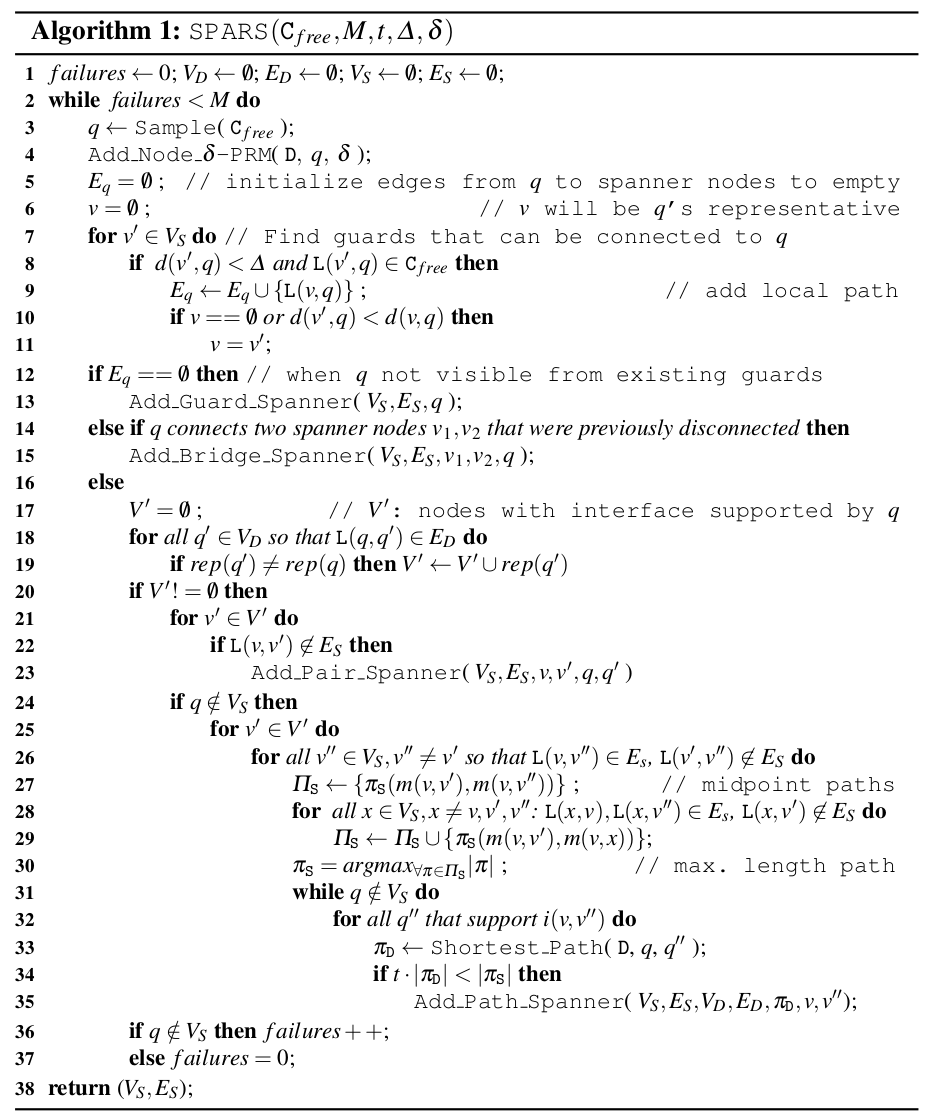
\includegraphics[width=0.49\textwidth]{spars}
\caption{SPARS pseudocode}
\end{figure}

The pros of the SPARS planner:
-highly efficient
-highly generalizable
-small solution plans
-probabilistically complete
-optimal solutions
-does not grow out of memory like other methods

The cons of the SPARS planner:
-maintains two graphs to meet completeness and optimality criteria
-inefficiencies fixed in SPARS2 planner

\subsection{SPArse Roadmap Spanner Algorithm Two} \label{SPARS2}
The SPARS2 planner was introduced as a simplification of the SPARS algorithm in \cite{spars_two}. As the SPARS planner uses two graphs to meet probabilistic 
completeness and near-optimality criteria, the SPARS2 planner reveals it is possible to relax the sampling conditions without using a dense graph. Desirable properties
of the SPARS algorithm are maintained in SPARS2, such as the decrease in probability to zero of adding new nodes to the roadmap over time. The SPARS2 algorithm
generates graphs that are orders of magnitude smaller than the PRM*-based solutions. Hence, the SPARS2 algorithm is competitively performant between the other sampling-
based approaches to path planning. The SPARS2 pseudocode can be found in figure 8.

\begin{figure}
\label{figure8} 
\centering 
\includegraphics[width=0.49\textwidth]{spars_two}
\caption{SPARS2 pseudocode}
\end{figure}

The upsides of the SPARS2 planner:
-pros of SPARS
-small growth rate and solution size, even less than SPARS

The downsides of the SPARS2 planner:
-compromise in final spanner size as compared to SPARS spanner

\subsection{Path-Directed Subdivision Trees} \label{PDST}
The PDST planner was designed specifically for systems with inherent drift, under-actuation and discrete changes. The approach utilizes a sampling-based
approach and path-directed subdivision to solve complex planning problems. The approach was proposed and applied in \cite{pdst} to the game Koules, which exhibits 
dynamical characteristics of complex motion planning problems. The algorithm was applied to scenarios with up to 85 dimensions, but obviously suffered from
memory overhead issues. Hence, the PDST is slower as memory size grows due to usage of hard disk page file and other hardware limitations, but the algorithm
should be applicable to a lower dimensional motion planning problem as for the turtlebot benchmark scenarios in this paper. The pseudocode for the algorithm is displayed in figure 9.

\begin{figure}
\label{figure9} 
\centering 
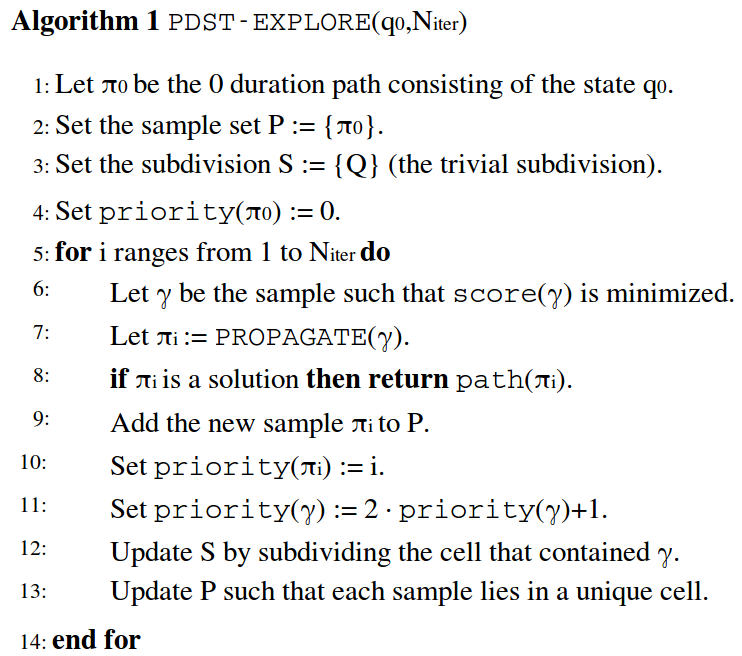
\includegraphics[width=0.49\textwidth]{pdst}
\caption{PDST pseudocode}
\end{figure}

Good features of the PDST algorithm follow:
-good for severe under-actuation
-good for significant drift
-good for high dimensionality
-appropriate for discrete system changes that occur at boundary conditions
-applicable to systems which are not reducible to a system with lower order dynamics

Bad features of the PDST algorithm follow:
-high state complexity
-requires path sampling representation for efficiency sake
-once the number of states needed to represent the search tree exceeds the size of the virtual memory, the speed decreases significantly due to disk accesses

\subsection{Fast Marching Tree Star} \label{FMT*}
The FMT* algorithm is a sampling-based planning algorithm that is targeted to solve complex motion planning problems in high-dimensional configuration space. The
algorithm is shown to be faster than both of its RRT* and the PRM* rivals. Unlike the other planners, the FMT* utilizes a lazy and recursive dynamic programming 
strategy to grow a tree of paths from a preselected number of probabilistically-drawn sample nodes. By doing this, it combines the features of both single and multi-
query path planners. It is influenced by the Fast Marching Method for solving Eikonal equations. It is described in \cite{fmt_star} and analyzed under the
notion of probability of convergence rather than analysis of sure converge like other planners. The convergence rate is bounded in big-O time and the algorithm
is found to be asymptotically-optimal even with various factors such as non-uniformly sampled nodes. The algorithm is found to generate much better solutions
that its RRT and PRM counterparts mostly in higher-dimensional configuration spaces or where collision-checking is inefficient. In figure 10 is the FMT* pseudocode.

\begin{figure}
\label{figure10} 
\centering 
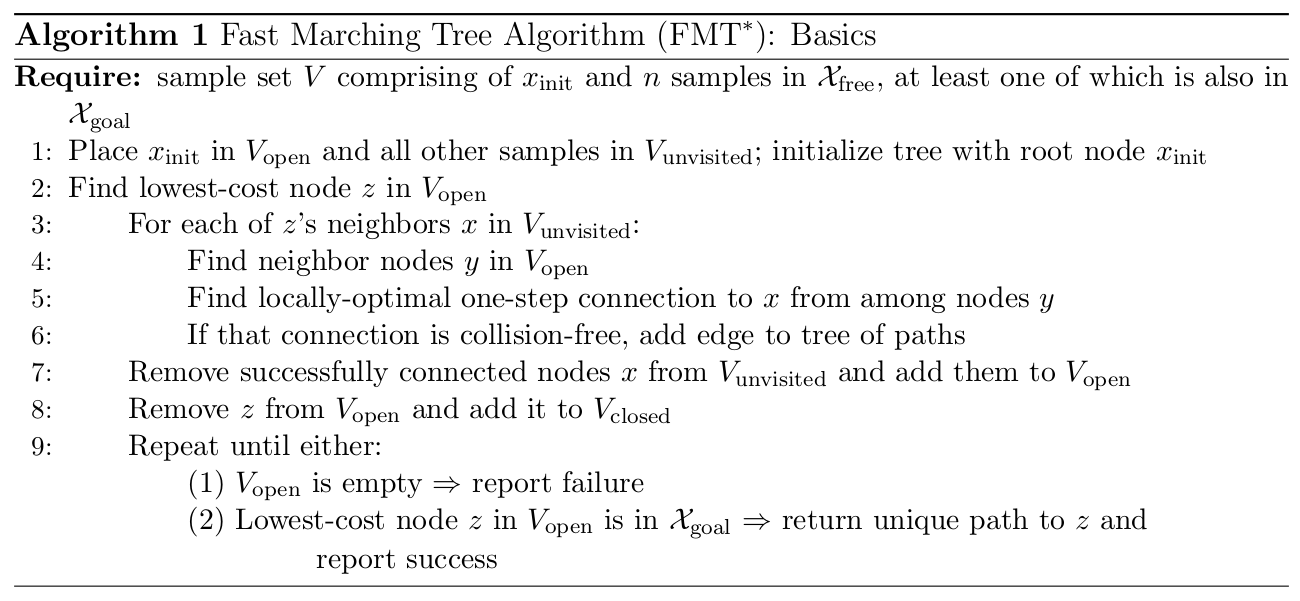
\includegraphics[width=0.49\textwidth]{fmt_star}
\caption{FMT* pseudocode}
\end{figure}

The beneficial aspects of the FMT* algorithm are the following:
-faster than the PRM*
-builds paths in a tree-like structure rather than a graph like PRM
-satisfies differential constraints in a forward fashion unlike graph-based algorithms (PRM)
-higher quality and more consistent solutions than RRT* given the uniformly larger error bars on the RRT* versus FMT* solution
-optimal without obstacles

The detrimental aspects of the FMT* algorithm are the following:
-only nearly optimal with obstacles


\subsection{Search Tree with Resolution Independent Density Estimation} \label{STRIDE}
The STRIDE algorithm was designed to support rapidly-exploring path planning in high-dimensional space with over 10 dimensions. The algorithm was first introduced
in \cite{stride}. The algorithm is mostly parameter-free due to the utilization of a Geometric Near-neighbor access tree (GNAT) to estimate the sampling density of the 
configuration space. This results in an implicitly resolution-independent Voronoi partitioning scheme to provide sampling density estimates, guiding the planner 
naturally to unexplored regions of configuration space. STRIDE is also capable of exploring the full dimensionality of the search space given that GNAT only requires a 
valid distance metric. Results in \cite{stride} show that the algorithm performs much better than others like the RRT and PRM when the search space is defined
by narrow passageways. Thus, the algorithm seems an appropriate match for a motion planning problem where tight passageways are common as in autonomous navigation.
Pseudocode for the algorithm is displayed in figure 11.

\begin{figure}
\label{figure2} 
\centering 
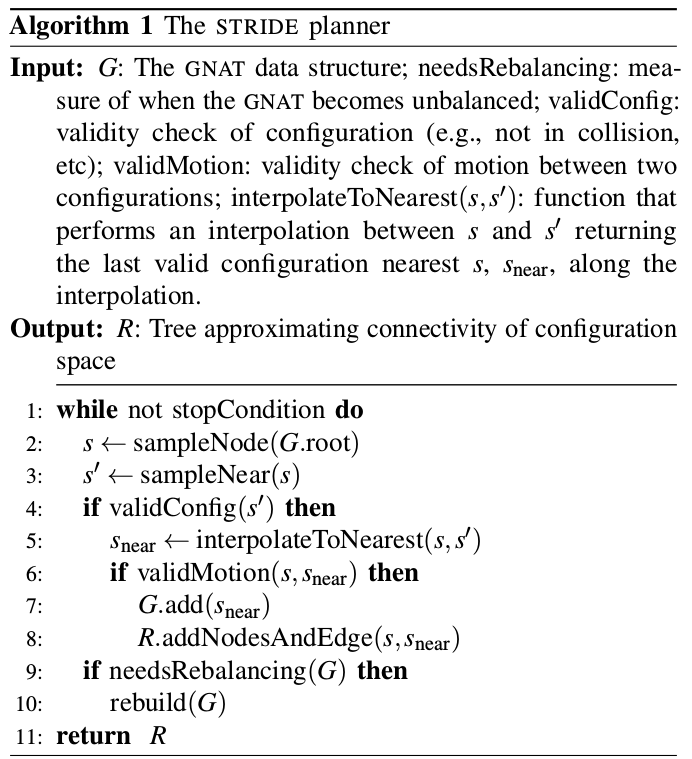
\includegraphics[width=0.49\textwidth]{stride}
\caption{STRIDE pseudocode}
\end{figure}

The best features of the STRIDE algorithm are:
-Voronoi partiitoning scheme
-resolution independent
-rapid exploration of unexplored regions
-performance improvements over other similar planners
-uses a data structure that enables it to produce density estimates fully in configuration space
-much more efficient than other planners
-smaller solution paths
-shorter runtime

The worst features of the STRIDE algorithm are:
-not guaranteed optimal
-not guaranteed probabilistically complete


\section{Benchmark Scenarios} \label{Benchmark Scenarios}

\subsection{Obstacle-Free Path} \label{Obstacle-free Path}

\subsection{Sparse Obstacle Map} \label{Sparse Obstacle Map}

\subsection{Dense Obstacle Map} \label{Dense Obstacle Map}

\section{Benchmark Comparisons} \label{Benchmark Comparison}

\subsection{Efficiency Comparisons} \label{Efficiency Comparisons}

\subsection{Performance Comparisons} \label{Performance Comparisons}

\section{Results} \label{Results}

\section{Conclusion} \label{Conclusion}

\subsection{Future Work}

\printbibliography
\end{document}